\documentclass[border=10pt]{standalone}
\usepackage{pgfplots}
\pgfplotsset{compat=1.18}
\begin{document}
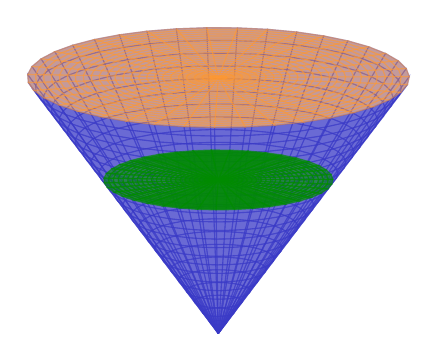
\begin{tikzpicture}
\begin{axis}[
    view={45}{18},
    axis lines=none,
    xlabel={$x$}, ylabel={$y$}, zlabel={$z$},
    domain=0:2, y domain=0:360, samples=25, samples y=40,
    zmin=0, zmax=2.4]
    % Cone surface z = r
    \addplot3[surf, shader=flat, opacity=0.5, color=blue!55!gray] ({x*cos(y)}, {x*sin(y)}, {x});
    % Top disk z = h
    \addplot3[surf, shader=flat, opacity=0.4, color=orange!80] ({x*cos(y)}, {x*sin(y)}, {2});
    % Typical cross-section disk at z = 1.2, radius 1.2
    \addplot3[surf, shader=flat, opacity=0.6, color=green!55!black] ({0.6*x*cos(y)}, {0.6*x*sin(y)}, {1.2});
\end{axis}
\end{tikzpicture}
\end{document}